% Reusable captions for teaching plates. Page 1 can be embedded in the appendix independently of the four main figures.
% Requires graphicx. The page option selects one plate of the two-page PDF.
\begin{figure}[tbp]
\centering
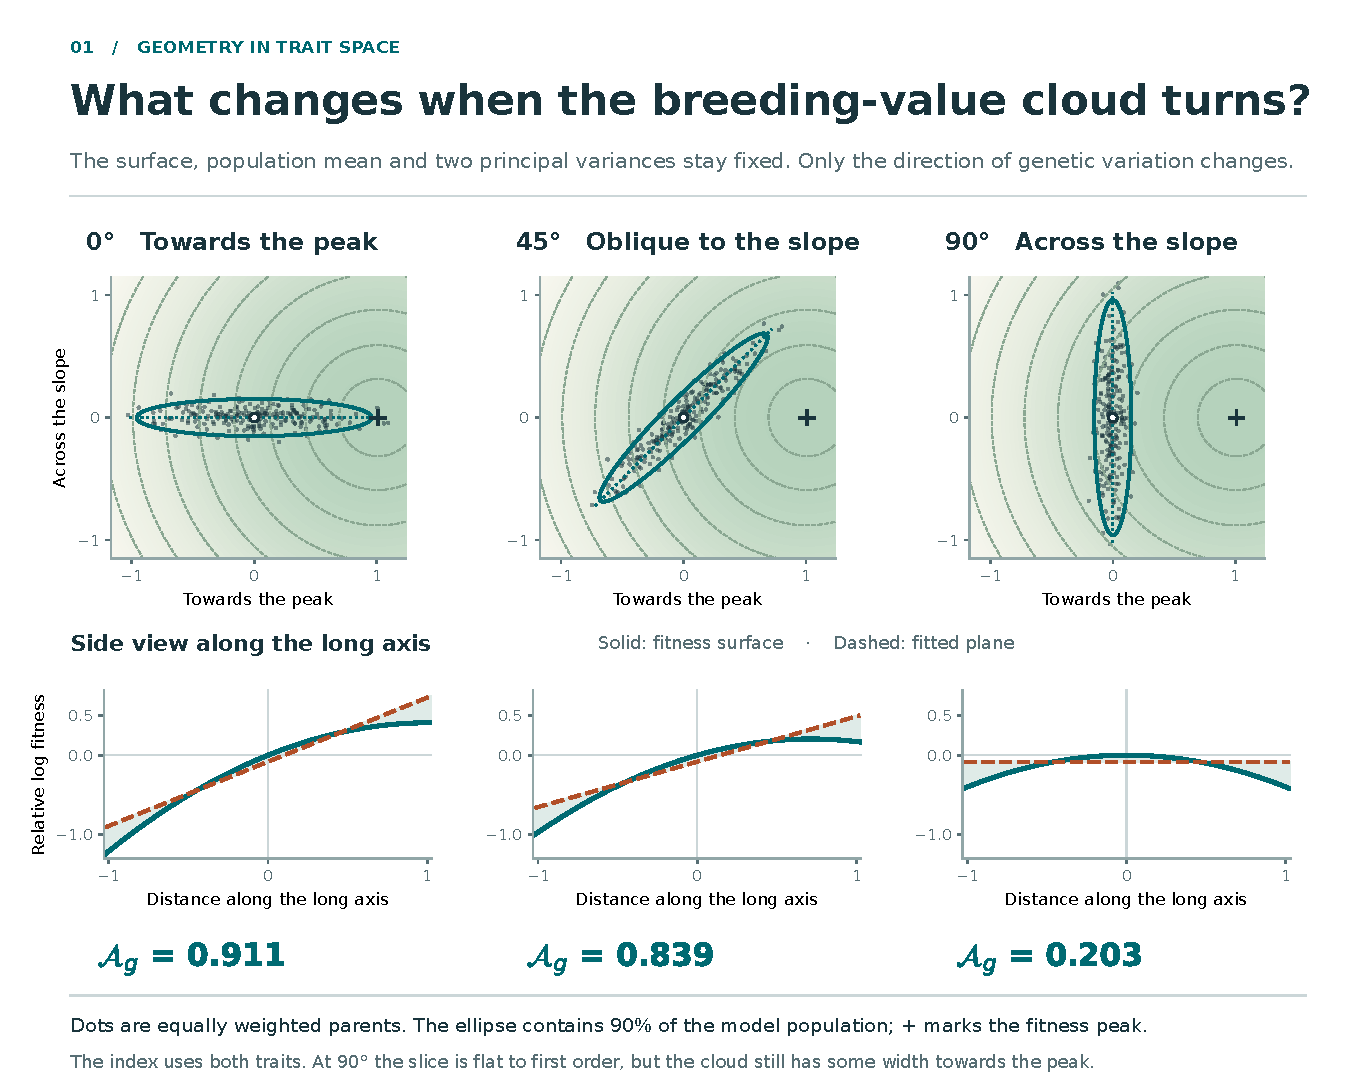
\includegraphics[page=1,width=\linewidth]{figures/geometry_of_additive_channels.pdf}
\caption{Rotating a breeding-value cloud on one fitness surface. Each dot represents a simulated parent; the two axes give its breeding values in coordinates that point towards and across the fitness peak. The ellipse encloses 90\% of the Gaussian population. The contours join breeding values at equal log expected fitness. From left to right, the same cloud turns through $0^\circ$, $45^\circ$ and $90^\circ$. Its mean, shape and size stay fixed. Below each map, the solid curve gives log expected fitness along the long axis, relative to the value at the mean. The dashed line gives the same section through the plane fitted to all parents. Because this landscape curves equally in every direction, the curvature variance stays fixed as the cloud turns. The linear variance falls as less genetic variation lies along the local log-fitness gradient. The linear share $\mathcal A_g$ falls from 0.911 to 0.203. It remains positive at $90^\circ$ because the cloud still has some width in the direction towards the peak. The dots illustrate the population; the calculations use its full distribution.}
\label{fig:ag-geometry-rotation}
\end{figure}

\begin{figure}[tbp]
\centering
\includegraphics[page=2,width=\linewidth]{figures/geometry_of_additive_channels.pdf}
\caption{The variance share as a projection. For a Gaussian population on this quadratic surface, the fitted plane and the remaining curvature give uncorrelated contributions to log expected fitness. Their standard deviations form the legs of a right triangle. With total standard deviation scaled to one, the squared base length is $\mathcal A_g$. At the peak the base vanishes and the displayed right angle is a limiting construction. Populations B and D have the same linear share but differ in their response to reproductive weighting. The diamond shows the change in mean parental breeding value when contributions follow the curved surface; the triangle gives the prediction from the fitted plane. Both changes are Euclidean distances in the same trait units. Percentages give the excess of the predicted distance over the distance on the curved surface.}
\label{fig:ag-geometry-projection}
\end{figure}
